\documentclass[usenames,dvipsnames,aspectratio=169]{beamer}
\usepackage[utf8]{inputenc}
\usepackage[spanish]{babel}
\usepackage{csquotes}
\usepackage[skip=0pt]{caption}
\captionsetup[figure]{labelformat=empty}
\usepackage{booktabs}
\usepackage{tabularx, colortbl}
\usepackage{setspace}
\usepackage{hyperref}
\usetheme{uniud}

%%% Some useful commands
% pdf-friendly newline in links
\newcommand{\pdfnewline}{\texorpdfstring{\newline}{ }} 
% Fill the vertical space in a slide (to put text at the bottom)
\newcommand{\framefill}{\vskip0pt plus 1filll}
\renewcommand{\emph}[1]{\textbf{\textcolor{UniGold}{#1}}}


\title[N-Reinas]{{\Large Sistemas Inteligentes}\\[0.2cm]Práctica 1: N-Reinas}

\date[Febrero, 2022]{Febrero de 2023}
\author[Aurora Esteban]{\texorpdfstring{
    \begin{minipage}{0.47\linewidth}
        Aurora Esteban Toscano
        \pdfnewline
        \texttt{aestebant@uco.es}
    \end{minipage}
    \hfill
    \begin{minipage}{0.47\linewidth}
        José Manuel Alcalde Llergo
        \pdfnewline
        \texttt{i72alllj@uco.es}
    \end{minipage}}{Aurora Esteban Toscano}
}
\institute{Grado en Ingeniería Informática, Universidad de Córdoba}
\begin{document}

\begin{frame}
\titlepage
\end{frame}

\begin{frame}{Objetivo}
	Poner en práctica las técnicas de búsqueda vistas en teoría sobre un problema clásico: \textbf{el puzzle de las N-Reinas}.
	\begin{itemize}
		\item Entender conceptualmente el problema de las N-Reinas.
		\item Entender el modelo de representación de estados que se proporciona.
		\item Implementar una técnica de búsqueda para resolver el problema.
		\item Utilizar la solución programada para responder al cuestionario \textbf{al final de clase}.
	\end{itemize}
\end{frame}

\begin{frame}{Fundamentos del problema I}
El problema de las N-Reinas consiste en colocar $n$ reinas en un tablero de dimensiones $n\times n$ de forma que no se amenace ninguna a otra $\rightarrow$ que no compartan fila, columna o diagonal.
\begin{figure}
	\centering
	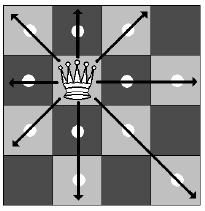
\includegraphics[width=.3\linewidth]{graphics/atacar.jpg}
	\caption{Posibles ataques de una reina en ajedrez}
\end{figure}
\end{frame}

\begin{frame}{Fundamentos del problema II}
El caso específico de las \textit{8 reinas} fue propuesto por el ajedrecista alemán Max Bezzel en 1848. Hoy en día se usa para explicar diversas técnicas de computación.
	\begin{minipage}{.6\linewidth}
		\begin{itemize}
			\item Definido para todos los números naturales.
			\item Los casos de $n=2$ y $n=3$ no tienen solución.
			\item Se sabe el número completo de soluciones hasta $n=27$.
			\item Los algoritmos de búsqueda por fuerza bruta pueden manejar variantes hasta $n\approx20$.
			\item Más allá, el coste computacional crece demasiado.
		\end{itemize}
	\end{minipage}
	\begin{minipage}{.35\linewidth}
		\begin{figure}
		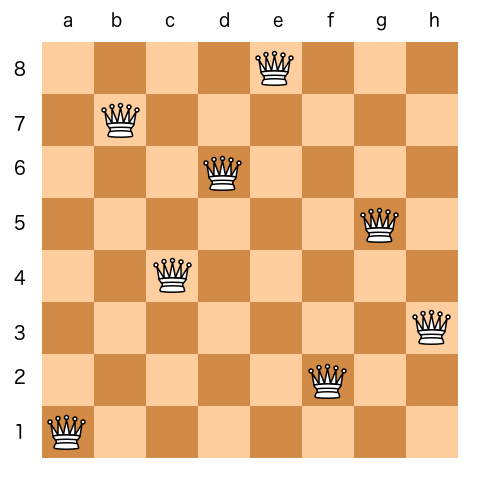
\includegraphics[width=.9\linewidth]{graphics/8queens.png}
		\caption{Una solución para $n=8$}
		\end{figure}
	\end{minipage}
\end{frame}

\begin{frame}{Material de la práctica}
	Para resolver el problema se proporciona una librería que funciona \textit{prácticamente}. Será necesario \textbf{hacer uso de las funciones que se proporcionan} para programar la técnica de búsqueda apropiada.
	\begin{itemize}
		\item \texttt{main.cpp}: fichero con la estructura principal del código. Tiene instrucciones para completar las tareas de programación.
		\item \texttt{State.h}: declaración de funciones genéricas para cualquier estado. En la solución deben usarse \texttt{isObjective()} y \texttt{getSucessors()}
		\item \texttt{QueensState-XXX.o}: librería pre-compilada con el código de funcionamiento interno de la librería. Dependiente de la arquitectura en la que se esté realizando la práctica.
	\end{itemize}
\end{frame}

\begin{frame}{Compilación y ejecución}
	\begin{enumerate}
		\item Compilar el programa según el SO:
		\begin{itemize}
			\item Ubuntu o equivalente: \texttt{g++ -o queensProf main.cpp QueensState-ubuntu.o}
			\item MacOS: \texttt{g++ -o queensProf main.cpp QueensState-macOS.o}
			\item LinuxUCO: \texttt{g++ -o queensProf main.cpp QueensState-aulasUCO.o}
		\end{itemize}
		\item Ejecutar el archivo creado: \texttt{./queensProf}.
			\begin{itemize}
				\item Recordar darle los permisos adecuados: \texttt{chmod u+x queensProf}
			\end{itemize}
	\end{enumerate}
	\begin{figure}
		\centering
		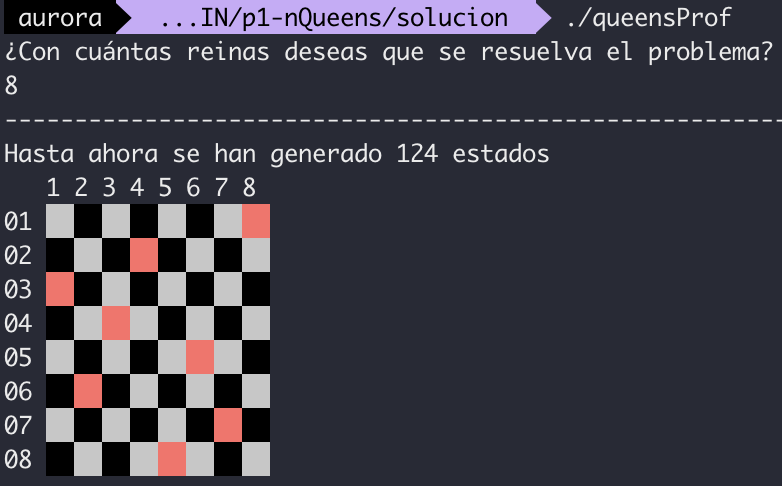
\includegraphics[width=.45\linewidth]{graphics/ejecucion.png}
	\end{figure}
\end{frame}

\begin{frame}{Tareas a implementar}
	\begin{itemize}
		\item Haciendo uso de la clase \texttt{stack} de C++:
		\begin{enumerate}
			\item Crear la estructura frontera.
			\item Insertar el estado inicial.
			\item Crear el bucle de búsqueda.
			\item Obtener el estado de frontera.
			\item Comprobar si es solución.
			\item Si no lo es, generar los sucesores e insertarlos en la frontera.
			\item Borrar el vector de sucesores de la memoria.
		\end{enumerate}
		\item Adicionalmente, tratar de cambiar el programa para implementar la frontera con una \textit{cola} en lugar de una pila.
	\end{itemize}
\end{frame}

\begin{frame}{Evaluación}
	En los últimos 10 minutos de clase se realizará un cuestionario de cuatro preguntas en Moodle para evaluar la práctica.
	
	Se necesitará ejecutar tanto el programa basado en pila como el basado en cola.
	\begin{itemize}
		\item Se recomienda conservar ambos ejecutables con distintos nombres para ejecutarlos rápidamente con las condiciones que se pidan.
	\end{itemize}
\end{frame}

\begin{frame}
\titlepage
\end{frame}
\end{document}